 \documentclass[aspectratio=169]{beamer}

% Must be loaded first
\usepackage{tikz}
\usetikzlibrary{shapes,arrows}

\usepackage[utf8]{inputenc}
\usepackage{textpos}

% Font configuration
\usepackage{fontspec}

\usepackage[listings, minted]{tcolorbox}
\usepackage{smartdiagram}
\usepackage[export]{adjustbox}

\input{font.tex}

% Tikz for beautiful drawings
\usetikzlibrary{mindmap,backgrounds}
\usetikzlibrary{arrows.meta,arrows}
\usetikzlibrary{shapes.geometric}

% Minted configuration for source code highlighting
\usepackage{minted}
\setminted{highlightcolor=orange!50, linenos}
\setminted{style=lovelace}

\usepackage[listings, minted]{tcolorbox}
\tcbset{left=6mm}

% Use the include theme
\usetheme{codecentric}

\newcommand{\emoji}[1]{
  \includegraphics[width=6mm, valign=c]{static-images/#1.png}
}

% Metadata
\title{Beautiful Composition}
\author{Markus Hauck}

% The presentation content
\begin{document}

\begin{frame}[noframenumbering,plain]
  \titlepage{}
\end{frame}

\section{Introduction}\label{sec:introduction}

\begin{frame}
  \frametitle{Compose This}
  \begin{itemize}
  \item what is the composition of
  \end{itemize}
\end{frame}

\begin{frame}
  \frametitle{Just Imagine}
  \begin{itemize}
  \item a world where your abstractions just fit together
  \item like lego blocks
  \item combinations everywhere
  \end{itemize}
\end{frame}

\begin{frame}
  \frametitle{Beautiful Composition \textemdash{} Themes}
  {
    \smartdiagramset{
      set color list={beamer@centricgreen!80,beamer@codeblue!80,red!50},
      module minimum width=3cm,
      text width=2.8cm
    }
    \smartdiagram[circular diagram]{
      Principle of Least Power,
      Composable Abstractions
    }
  }
  \begin{itemize}
  \item Themes in this presentation:
  \item design: the principle of least power
  \item important property of an abstraction: composition
  \end{itemize}
\end{frame}

\begin{frame}[fragile]
  \frametitle{Content}
  \begin{center}
    \resizebox{!}{0.8\textheight}{
      \smartdiagram[bubble diagram]{
        Content,
        2 Monoids,
        1 Introduction,
        5 Conclusion,
        4 Streaming,
        3 Applicatives
      }
    }
  \end{center}
\end{frame}

\begin{frame}
  \frametitle{The Principle Of Least Power}
    \begin{tcolorbox}[
      fonttitle=\sffamily\bfseries,
      colbacktitle=black,
      colframe=black,
      coltitle=beamer@centricgreen,
      title=The Principle
      ]
      ``\ldots{} picking not the most powerful solution but the least powerful''
  \end{tcolorbox}
  \begin{itemize}
  \item https://www.w3.org/DesignIssues/Principles.html
  \item same is valid for abstractions from functional programming
  \item if you don't need Monad, don't require it
  \end{itemize}
  \vfill
  \begin{quote}
    The reason for this is that the \textbf{less powerful} the language, \textbf{the
      more} you can do with the \textbf{data} stored\ldots
  \end{quote}
\end{frame}

\begin{frame}
  \frametitle{Composition}
  \begin{itemize}
  \item abstractions help to hide details and reason at a higher level
  \item real power comes when those abstractions compose
  \item otherwise isolated island you have to throw over board
  \item most ``classic'' GoF Design Patterns in OO fail to compose
  \item many ``mathematical'' abstractions in FP compose naturally
  \item example: inductive monoid, product of monoids (more later)
  \item leaky abstraction (TODO: include?)
  \end{itemize}
\end{frame}

\begin{frame}
  \frametitle{The Case Study}
  \begin{itemize}
  \item we want to analyze text
  \item collect metrics
  \item single traversal
  \end{itemize}

  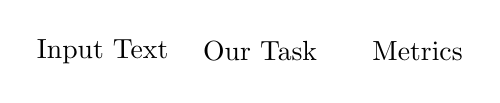
\begin{tikzpicture}[node distance = 20mm, auto]
    \tikzstyle{box} = [rectangle, draw, text centered, rounded corners, minimum width=6mm, minimum height=6mm]

    \node [box, draw=none] (text) {Input Text};
    \node [box, draw=none, right of=text] (blackbox) {Our Task};
    \node [box, draw=none, right of=blackbox] (metrics) {Metrics};
  \end{tikzpicture}
\end{frame}

\begin{frame}[fragile]
  \frametitle{A First Solution}
  \inputminted[fontsize=\small]{scala}{snippets/imperative-wc.scala}
\end{frame}

\begin{frame}
  \frametitle{Metrics}
  \begin{itemize}
  \item number of chars (count each char)
  \item number of lines (count newline characters)
  \item number of words (harder, because it is context sensitive)
  \item open for extension (closed for modification)
  \end{itemize}
\end{frame}

\section{Monoids}\label{sec:monoids}

\begin{frame}
  \frametitle{Let's Get Our FP Tools!}
  % image of toolset?
\end{frame}

\begin{frame}[fragile]
  \frametitle{Monoids}
  \begin{itemize}
  \item Quick Recap: Monoids
  \item binary method \texttt{combine} and nullary method \texttt{combine}
    \begin{minted}{scala}
      trait Monoid[A] {
        def combine(x: A, y: A): A
        def empty: A
      }
    \end{minted}
  \end{itemize}
\end{frame}

\begin{frame}
  \frametitle{Monoids: Basic Idea}
  \begin{itemize}
  \item basic approach: iterate over all \texttt{Char} and accumulate using a monoid
  \end{itemize}
\end{frame}

\begin{frame}[fragile,t]
  \frametitle{Monoids: Counting Chars}
  \begin{itemize}
  \item counting chars is easy, use \texttt{(Int, +)} as a Monoid
  \item count 1 (\texttt{mappend} 1) for every character
  \end{itemize}
  \vspace{1cm}
  \begin{tikzpicture}[node distance = 8mm, auto]
    \tikzstyle{box} = [rectangle, draw, text centered, rounded corners, minimum width=6mm, minimum height=6mm]
    \tikzstyle{mon} = [rectangle, draw, text centered, minimum width=25mm, minimum height=6mm, fill=red!10]
    \tikzstyle{line} = [draw, -latex']

    \node [box, draw=none] (a0) {};
    \node [box, draw=none, left of=a0] (dummy) {};

    \foreach \char [count=\pos, evaluate=\pos as \i using int(\pos-1)] in {h,e,l,l,o,\textbackslash{n},w,o,r,l,d,!,\textbackslash{n}} {
      \ifthenelse{\isodd{\pos}}{
        \node [box, fill=beamer@codeblue!70, right of=a\i] (a\pos) {\char};
      }{
        \node [box, fill=beamer@centricgreen!70, right of=a\i] (a\pos) {\char};
      }
      \only<\pos>{
        \node [mon, below of=a\pos, yshift=-5mm] (b\pos) {\i\ + 1 = \pos};
        \path [line] (b\pos) -- (a\pos);
      }
    }
  \end{tikzpicture}

  \vfill
  \only<13>{
    \begin{itemize}
    \item so the result is 13 chars in total
    \end{itemize}
  }
\end{frame}

\begin{frame}[fragile, t]
  \frametitle{Monoids: Counting Chars}
  \begin{itemize}
  \item to count lines, use again \texttt{(Int, +)} as a Monoid
  \item but \textbf{only} count 1 if the character is a \textbackslash{n}
  \end{itemize}
  \vspace{1cm}
  \begin{tikzpicture}[node distance = 8mm, auto]
    \tikzstyle{box} = [rectangle, draw, text centered, rounded corners, minimum width=6mm, minimum height=6mm]
    \tikzstyle{mon} = [rectangle, draw, text centered, minimum width=25mm, minimum height=6mm, fill=red!10]
    \tikzstyle{line} = [draw, -latex']

    \node [box, draw=none] (a0) {};
    \node [box, draw=none, left of=a0] (dummy) {};

    \foreach \char [count=\pos, evaluate=\pos as \i using int(\pos-1)] in {h,e,l,l,o,\textbackslash{n},w,o,r,l,d,!,\textbackslash{n}} {
      \ifthenelse{\isodd{\pos}}{
        \node [box, fill=beamer@codeblue!70, right of=a\i] (a\pos) {\char};
      }{
        \node [box, fill=beamer@centricgreen!70, right of=a\i] (a\pos) {\char};
      }
      \only<\pos>{
        \ifthenelse{\pos > 5}{
          \ifthenelse{\pos > 12}{
            \node [mon, below of=a\pos, yshift=-5mm] (b\pos) {1\ + 1 = 2};
          }{
            \ifthenelse{\pos = 6}{
              \node [mon, below of=a\pos, yshift=-5mm] (b\pos) {0\ + 1 = 1};
            }
            {
              \node [mon, below of=a\pos, yshift=-5mm] (b\pos) {1\ + 0 = 1};
            }
          }
        }{
          \node [mon, below of=a\pos, yshift=-5mm] (b\pos) {0 + 0 = 0};
        }
        \path [line] (b\pos) -- (a\pos);
      }
    }
  \end{tikzpicture}

  \only<13>{
    \begin{itemize}
    \item we counted 2 lines in total
    \end{itemize}
  }
\end{frame}

\begin{frame}
  \frametitle{Composing Monoids}
  \begin{itemize}
  \item for multiple metrics, do multiple passes?!
  \item no \textemdash{} because monoids \textbf{compose}
    \begin{itemize}
    \item inductive: monoid + base monoid
    \item product: tuple of monoids
    \end{itemize}
  \end{itemize}
\end{frame}

\begin{frame}
  \frametitle{Monoid Composition \textemdash{} Induction}
  \begin{itemize}
  \item some Monoids are based inductively on others
  \item Option, Future, IO, Task, \ldots{}
  \end{itemize}
\end{frame}

\begin{frame}[fragile]
  \frametitle{Monoid Composition \textemdash{} Option And Stopwords}
  \begin{itemize}
  \item as an example: filter out (don't count) stopwords
  \item stopwords = most common words that are not interesting (``the'', ``a'', \ldots{})
  \item the Option-Monoid works like this:
  \end{itemize}
  \begin{center}
  \begin{minted}{scala}
None |+| y === y
x |+| None === x
Some(x) |+| Some(y) === Some(x |+| y)
  \end{minted}
\end{center}
\end{frame}

\begin{frame}[fragile]
  \frametitle{Monoid Composition \textemdash{} Option And Stopwords}
  \begin{itemize}
  \item idea: if it is a stopword, use None, otherwise regular count with Some
  \end{itemize}
  \begin{center}
  \begin{minted}{scala}
None |+| y === y
x |+| None === x
Some(x) |+| Some(y) === Some(x |+| y)
  \end{minted}
\end{center}
\end{frame}

\begin{frame}[fragile]
  \frametitle{Monoid Composition \textemdash{} Option And Stopwords}
  \begin{itemize}
  \item assuming both ``is'' and ``a'' are classified as stopwords:
  \end{itemize}
  \vspace{1cm}
  \begin{tikzpicture}[node distance = 15mm, auto]
    \tikzstyle{box} = [rectangle, draw, text centered, rounded corners, minimum width=6mm, minimum height=6mm]
    \tikzstyle{mon} = [rectangle, draw, text centered, minimum width=25mm, minimum height=6mm, fill=red!10]
    \tikzstyle{line} = [draw, -latex']

    \node [box, draw=none] (a0) {};
    \node [box, draw=none, left of=a0] (dummy) {};

    \foreach \word [count=\pos, evaluate=\pos as \i using int(\pos-1)] in {this,is,a,test,text} {
      \ifthenelse{\isodd{\pos}}{
        \node [box, fill=beamer@codeblue!70, right of=a\i] (a\pos) {\word};
      }{
        \node [box, fill=beamer@centricgreen!70, right of=a\i] (a\pos) {\word};
      }
      \only<\pos>{
        \ifthenelse{\pos = 2 \OR \pos = 3}{
          \node [mon, below of=a\pos, yshift=-5mm] (b\pos) {Some(1)\ |+| None = Some(1)};
        }{
          \ifthenelse{\pos = 1}{
            \node [mon, below of=a\pos, yshift=-5mm] (b\pos) {None\ |+| Some(1) = Some(1)};
          }{
            \ifthenelse{\pos=4}{
              \node [mon, below of=a\pos, yshift=-5mm] (b\pos) {Some(1)\ |+| Some(1) = Some(2)};
            }{
              \node [mon, below of=a\pos, yshift=-5mm] (b\pos) {Some(2)\ |+| Some(1) = Some(3)};
            }
          }
        }
        \path [line] (b\pos) -- (a\pos);
      }
    }
  \end{tikzpicture}
  \vspace{1cm}
  \begin{itemize}
  \item<5> count without stopwords is 3
  \end{itemize}
\end{frame}

\begin{frame}
  \frametitle{Monoid Composition \textemdash{} Option And Stopwords}
  \begin{itemize}
  \item just an example, more options:
    \begin{itemize}
    \item don't count chars like \texttt{!?,.} etc.\ using Option again
    \item use \texttt{Future/Task/IO} to get parallelism
    \item and so much more
    \end{itemize}
  \end{itemize}
\end{frame}

\begin{frame}
  \frametitle{Monoid Composition \textemdash{} Induction}
  \begin{itemize}
  \item base instance does not have to be a Monoid
  \item using \texttt{Option} we can lift any \texttt{Semigroup}
  \item \texttt{empty} becomes \texttt{None}
  \end{itemize}
\end{frame}

\begin{frame}
  \frametitle{Monoid Composition \textemdash{} Tuple}
  \begin{itemize}
  \item if \texttt{A} and \texttt{B} have a Monoid instance, so does \texttt{(A,B)}
  \item combine the two \texttt{A}'s and the two \texttt{B}'s
  \item we can fuse our two metrics!
  \end{itemize}
\end{frame}

\begin{frame}[fragile, t]
  \frametitle{Multiple Monoids \textemdash{} One Traversal}
  \vspace{15mm}
  \begin{tikzpicture}[node distance = 8mm, auto]
    \tikzstyle{box} = [rectangle, draw, text centered, rounded corners, minimum width=6mm, minimum height=6mm]
    \tikzstyle{mon} = [rectangle, draw, text centered, minimum width=25mm, minimum height=6mm, fill=red!10]
    \tikzstyle{line} = [draw, -latex']

    \node [box, draw=none] (a0) {};
    \node [box, draw=none, left of=a0] (dummy) {};

    \foreach \char [count=\pos, evaluate=\pos as \i using int(\pos-1)] in {h,e,l,l,o,\textbackslash{n},w,o,r,l,d,!,\textbackslash{n}} {
      \ifthenelse{\isodd{\pos}}{
        \node [box, fill=beamer@codeblue!70, right of=a\i] (a\pos) {\char};
      }{
        \node [box, fill=beamer@centricgreen!70, right of=a\i] (a\pos) {\char};
      }
      \only<\pos>{
        \ifthenelse{\pos > 5}{
          \ifthenelse{\pos > 12}{
            \node [mon, below of=a\pos, yshift=-5mm] (b\pos) {1\ + 1 = 2};
          }{
            \ifthenelse{\pos = 6}{
              \node [mon, below of=a\pos, yshift=-5mm] (b\pos) {0\ + 1 = 1};
            }
            {
              \node [mon, below of=a\pos, yshift=-5mm] (b\pos) {1\ + 0 = 1};
            }
          }
        }{
          \node [mon, below of=a\pos, yshift=-5mm] (b\pos) {0 + 0 = 0};
        }

        \node [mon, below of=b\pos, yshift=2mm] (c\pos) {\i\ + 1 = \pos};
        \node [mon, below of=c\pos, yshift=2mm] (d\pos) {\ldots{}};
        \path [line] (b\pos) -- (a\pos);
      }
    }
  \end{tikzpicture}
  \only<13>{
    \begin{itemize}
    \item result: \texttt{2} lines and \texttt{13} chars
    \end{itemize}
  }
\end{frame}

\begin{frame}
  \frametitle{More Monoids}
  \begin{itemize}
  \item for \texttt{wc} we have two of our three target metrics
  \item but actually, we can do a lot more than that!
    \begin{itemize}
    \item find longest word
    \item count occurrences by word
    \item average word length (as own monoid or derive)
    \end{itemize}
  \end{itemize}
\end{frame}

\begin{frame}
  \frametitle{Calculating With Monoids}
  \begin{itemize}
  \item adding things (or multiplying)
  \item min and max
  \item map of key to value (for any monoid as value)
  \item we can calculate our metrics with monoids
  \item chars is the integer monoid with addition
  \item lines is also the integer monoid, but only count 1 if char is a newline
  \item for words, for now just split the input and count 1 on every ``group''
  \end{itemize}
\end{frame}

\begin{frame}
  \frametitle{Wordcount (Monoids, Chars)}
  \inputminted[fontsize=\footnotesize]{scala}{snippets/wc-monoid-char.scala}
\end{frame}

\begin{frame}
  \frametitle{Wordcount (Monoids, Strings)}
  \inputminted[fontsize=\footnotesize]{scala}{snippets/wc-monoid-string.scala}
\end{frame}

\begin{frame}
  \frametitle{Monoids \textemdash{} Review}
  \begin{itemize}
  \item composes very well from small blocks
  \item easy to extend using custom metrics
  \item \texttt{Option} can lift any Semigroup
  \item works beautifully with everything that can be folded
  \end{itemize}
  \vspace{1cm}
  \inputminted[fontsize=\small]{scala}{snippets/foldable-def.scala}
\end{frame}

\section{Applicatives}\label{sec:applicatives}

\begin{frame}[fragile]
  \frametitle{From Monoids To Applicatives}
  \begin{itemize}
  \item also called \textbf{Monoidal} Functors
  \item ``monoidal'' in the effects (pure = ``empty'' effect, \texttt{<*>} = ``combine effects'')
  \end{itemize}
  \vfill
  \inputminted[fontsize=\small]{scala}{snippets/applicative-def.scala}
\end{frame}

\begin{frame}[fragile]
  \frametitle{Applicative as Effect Monoids}
  \begin{itemize}
  \item \texttt{Applicatives} adds richer structure, \textbf{monoidal} in effects
  \item \texttt{pure} is like \texttt{empty} \textit{for effects}
  \item \texttt{product}\footnote{from Semigroupal} is like \texttt{combine} \textit{for effects}
  \end{itemize}
  \begin{minted}{scala}
    def empty      : F
    def pure(x: A) : F[A]

    def combine( x: F,     y: F)   : F
    def product(fa: F[A], fb: F[B]): F[A]
  \end{minted}
\end{frame}

\begin{frame}
  \frametitle{No Monoids? \emoji{scream}}
  \begin{itemize}
  \item but wait a moment, was all we learned about Monoids for nothing?!
  \item rejoice, we can reuse \textbf{everything} we have until now
  \item actually two ways
    \begin{itemize}
    \item lift Monoid inside Applicative
    \item promote any Monoid to an Applicative
    \end{itemize}
  \end{itemize}
\end{frame}

\begin{frame}[fragile]
  \frametitle{Monoids Inside Applicatives}
  \begin{itemize}
  \item for every \texttt{F[A]}, given \texttt{Applicative[F]} and \texttt{Monoid[A]}
  \item we can define
  \end{itemize}

  \begin{minted}{scala}
    def empty: F[A] = pure(Monoid[A].empty)

    def combine(x: F[A], y: F[A]): F[A] =
      Applicative[F].map2(x, y)(Monoid[A].combine)
  \end{minted}
\end{frame}

\begin{frame}[fragile]
  \frametitle{The Const Datatype}
  \begin{center}
    \inputminted[fontsize=\small]{scala}{snippets/const-def.scala}
  \end{center}
  \vspace{1cm}
  \begin{itemize}
  \item simple case class with phantom type parameter
  \item \ldots{} and one actual value
  \item let's define \texttt{Functor} and \texttt{Applicative}
  \end{itemize}
\end{frame}

\begin{frame}[fragile]
  \frametitle{The Const Datatype}
  \begin{center}
    \inputminted[fontsize=\small]{scala}{snippets/const-try-applicative.scala}
  \end{center}
\end{frame}

\begin{frame}[fragile]
  \frametitle{The Const Datatype}
  \begin{center}
    \inputminted[fontsize=\small, highlightlines={1,8,12}]{scala}{snippets/const-applicative.scala}
  \end{center}
\end{frame}

\begin{frame}
  \frametitle{The Const Datatype}
  \begin{itemize}
  \item the functor instance is a little strange
  \item but the applicative instance is super awesome
  \item remember \texttt{Option} lifting any \texttt{Semigroup}?
  \item allows you to lift any \texttt{Monoid} into an \texttt{Applicative}!
  \item that means we can still use everything we already have
  \item (nb: Const is a monoid isomorphism)
  \end{itemize}
\end{frame}

\begin{frame}
  \frametitle{Composition And Applicatives}
  \begin{itemize}
  \item remember \texttt{Monoid} composition? Nesting and tupling
  \item we get the same for \texttt{Applicative} (from e.g.\ \texttt{cats})
    \begin{itemize}
    \item Nested
    \item Tuple2K
    \end{itemize}
  \item why is that a big deal again?
  \end{itemize}
\end{frame}

\begin{frame}[fragile]
  \frametitle{Composition And Applicatives}
  \inputminted[fontsize=\small]{scala}{snippets/compose-applicative-monoid.scala}
  \inputminted[fontsize=\small]{scala}{snippets/compose-applicative-1.scala}
\end{frame}

\begin{frame}[fragile]
  \frametitle{Composition And Applicatives}
  \inputminted[fontsize=\small]{scala}{snippets/compose-applicative-2.scala}
\end{frame}

\begin{frame}
  \frametitle{Traversing With Applicatives}
  \begin{itemize}
  \item for monoids, \texttt{foldMap} is the essential operation
  \item for applicatives, change to \texttt{traverse}
  \item we can derive \texttt{foldMap} from \texttt{traverse}
  \end{itemize}
  \vspace{1cm}
  \inputminted[fontsize=\small]{scala}{snippets/traverse-def.scala}
\end{frame}

\begin{frame}
  \frametitle{Metrics via Applicatives}
  \begin{itemize}
  \item using applicatives we have all the power we need
  \item use State, Task, IO, \ldots
  \end{itemize}
\end{frame}

\begin{frame}
  \frametitle{Counting Words \textemdash{} With State}
  \begin{itemize}
  \item we can re-use the counting of chars and lines (and any monoidal metric)
  \item as seen, have to be more clever for words
  \item idea: keep track of state: \textbf{inside} vs \textbf{outside} a word
  \item how to do this with applicatives?
  \item \textbf{State}, IO, ST, \ldots{}
  \end{itemize}
\end{frame}

\begin{frame}[fragile]
  \frametitle{Counting Words \textemdash{} With State}
  \inputminted[fontsize=\small]{scala}{snippets/count-words-state.scala}
\end{frame}

\begin{frame}
  \frametitle{Overview}
  \def\firstcircle{(0,0) ellipse (20mm and 5mm)}
  \def\secondcircle{(0,0) ellipse (25mm and 12mm)}
  \def\thirdcircle{(0,0) ellipse (35mm and 20mm)}
  \begin{center}
    \begin{tikzpicture}
      \begin{scope}[fill opacity=0.5]
        \fill[beamer@centricgreen!90] \firstcircle;
        \fill[beamer@codeblue!90] \secondcircle;
        \fill[red!5] \thirdcircle;
        \draw \firstcircle node  {$Semigroup$};
        \draw \secondcircle node [yshift=-8mm] {$Monoid$};
        \draw \thirdcircle node [yshift=-16mm] {$Applicative$};
      \end{scope}
    \end{tikzpicture}
  \end{center}
\end{frame}

\begin{frame}
  \frametitle{Monads Must Be Great!}
  \begin{itemize}
  \item if \texttt{Applicative} brings us so much power, how good must it be with \texttt{Monad}
  \item unfortunately, \texttt{Monad}s are not as good as they seem
  \item \texttt{Functor} and \texttt{Applicative} are \textbf{closed} under composition
  \item arbitrary nesting of \texttt{Functor} inside \texttt{Functor}
    / or \texttt{Applicative} inside \texttt{Applicative}
  \item \texttt{Monad} is \textbf{not} closed, not guaranteed to be a \texttt{Monad} at all!
  \item and Product (Tuple) does not work either
  \item \texttt{Monad}s are absolutely overrated
  \item see ``The Essence Of The Iterator Pattern'', section 5.4
  \end{itemize}
\end{frame}

\section{Streaming}\label{sec:streaming}

\begin{frame}
  \frametitle{Okay but traversing Lists/Iterators/etc is suboptimal!}
  \begin{itemize}
  \item but there is no \texttt{traverse} for real streams?!
  \item because there can't be one\ldots (why?)
  \item but: do we need the actual \texttt{traverse}
  \item realization: \texttt{traverse\_} (\texttt{Foldable}) is enough!
  \end{itemize}
\end{frame}

\begin{frame}
  \frametitle{Traverse and Foldable}
  \begin{itemize}
  \item so what's the difference between \texttt{traverse} and \texttt{traverse\_}
  \item the regular \texttt{traverse} keeps the whole structure!
  \item the \texttt{traverse\_} variant only secquences effects!
  \item important: Applicative effect sequencing is \textbf{associative} as per the laws
  \item that means we can work on the stream in parallel
  \end{itemize}
\end{frame}

\begin{frame}[fragile]
  \frametitle{Implement traverse\_ for fs2}
  \begin{itemize}
  \item our framework needs the \texttt{traverse\_}
  \item can be implemented for anything that has a proper \texttt{fold}
  \item let's do it for fs2 \texttt{Stream}
  \end{itemize}
  \vspace{1cm}
  \inputminted[fontsize=\small]{scala}{snippets/fs2-traverse-stream.scala}
\end{frame}

\begin{frame}[fragile]
  \frametitle{Counting Words With fs2}
  \begin{itemize}
  \item example uses fs2 (also possible: akka-streams)
  \end{itemize}
  \vspace{1cm}
  \inputminted[fontsize=\small]{scala}{snippets/fs2-count-words.scala}
\end{frame}

\begin{frame}
  \frametitle{Counting Words With Streams}
  \begin{itemize}
  \item suddenly we can use all the stream processing goodness
  \item we could chunk the input and process in parallel (but keep order)
  \item by carefully choosing the \texttt{Applicative}, operate with constant memory
  \item use existing connectors to read from DB, Kafka, etc.
  \item very flexible and almost for free!
  \end{itemize}
\end{frame}

\section{Conclusion}\label{sec:conclusion}

\begin{frame}
  \frametitle{Conclusion}
  \begin{itemize}
  \item we can add metrics easily
  \item control flow can be easily customized
  \item (sometimes) Monads are overrated
  \end{itemize}
\end{frame}

\begin{frame}
  \frametitle{Abstraction}
  \smartdiagramset{set color list={beamer@centricgreen!80,beamer@codeblue!80,red!50}}
  \smartdiagram[priority descriptive diagram]{
    Semigroup,
    Monoid,
    Applicative
  }
\end{frame}

\begin{frame}
  \frametitle{The End}
  \begin{itemize}
  \item \hyperref[sec:introduction]{Introduction}
  \item \hyperref[sec:monoids]{Monoids}
  \item \hyperref[sec:applicatives]{Applicatives}
  \item \hyperref[sec:streaming]{Streaming}
  \item \hyperref[sec:conclusion]{Conclusion}
  \end{itemize}
\end{frame}

\appendix{}

\begin{frame}
  \frametitle{Brand New: Selective Functors}
  \begin{itemize}
  \item like applicatives, we can use a product of selective functors
  \item example: find the index of a word
  \end{itemize}
\end{frame}

\end{document}
